% 2007 年湖北卷文科第 21 题：抛物线 x^2=2py，过 C(0,p) 的直线交于 A、B，
%   N 为 C 关于原点的对称点。
% 来源 PDF：gaokaomath-src/普通高考/2007/2007湖北文.pdf
% SHA-256：290a153da24ec0f3a3abb8bb916d9b7e06d203d3ef5bd7bb221c93f7f1b1cacb
% 原页：2007湖北文.pdf 第 2 页（A3 三栏）第 3 栏，书页码 378。
% 重绘依据：按原页抛物线、割线与 C、N 的位置重绘，p=1 仅作示意。
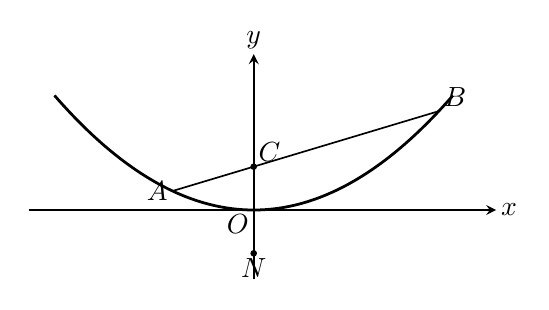
\begin{tikzpicture}[x=1.1cm, y=0.55cm, semithick,
  every node/.style={inner sep=1.5pt}]
  \draw[->,>=stealth] (-2.6,0) -- (2.8,0) node[right] {$x$};
  \draw[->,>=stealth] (0,-1.6) -- (0,3.6) node[above] {$y$};
  \node[below left] at (0,0) {$O$};

  \draw[domain=-2.3:2.3,samples=120,line width=1pt] plot (\x,{\x*\x/2});

  \coordinate (C) at (0,1);
  \coordinate (N) at (0,-1);
  \coordinate (A) at (-0.937,0.439);
  \coordinate (B) at (2.137,2.283);

  \draw (A) -- (B);
  \fill (C) circle (1.2pt);
  \fill (N) circle (1.2pt);
  \node[above right] at (C) {$C$};
  \node[below] at (N) {$N$};
  \node[left] at (A) {$A$};
  \node[above right] at (B) {$B$};
\end{tikzpicture}
